\documentclass[12pt]{article}

% Packages
\usepackage[utf8]{inputenc}
\usepackage{amsmath}
\usepackage{amssymb}
\usepackage{graphicx}
\usepackage{hyperref}
\usepackage{geometry}

% Geometry settings
\geometry{
    a4paper,
    total={170mm,257mm},
    left=20mm,
    right=20mm,
    top=20mm,
    bottom=20mm,
}

% Set the figure counter to reset within subsections
\counterwithin{figure}{subsection}

% Document
\begin{document}

% Title Page
\title{Homework 1: Vector Search}
\author{Naomi Derel 325324994, Gili Cohen 326280815, Renana Shachak}
\date{\today}
\maketitle

% % Table of Contents
% \tableofcontents
% \newpage

% Sections
\section{Faiss}

\subsection{Running Times}

\begin{figure}[h]
    \centering
    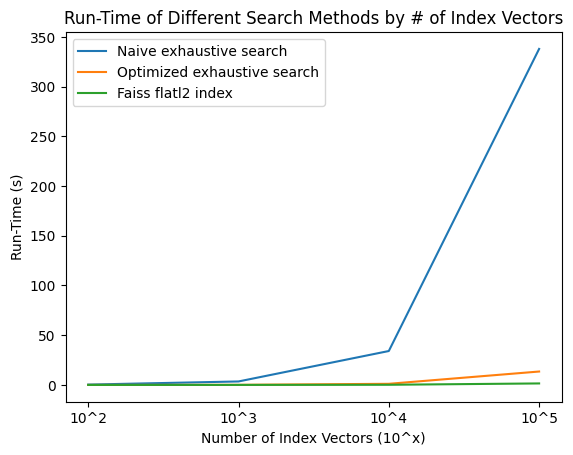
\includegraphics[width=0.5\textwidth]{images/1_1_1.png}
    \caption{Running times by Number of Index Vectors}
\end{figure}

\begin{figure}[h]
    \centering
    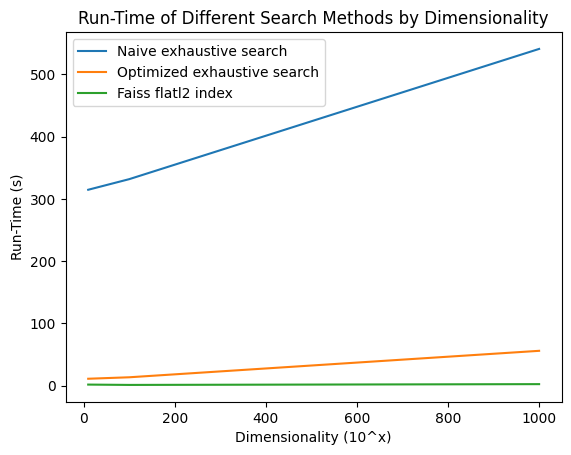
\includegraphics[width=0.5\textwidth]{images/1_1_2.png}
    \caption{Running times by Dimentionality}
\end{figure}

\subsection{Faiss LSH}



% % Bibliography
% \newpage
% \begin{thebibliography}{99}
%     \bibitem{ref1} Author, \emph{Title}, Publisher, Year.
%     \bibitem{ref2} Author, \emph{Title}, Publisher, Year.
%     % Add more references as needed
% \end{thebibliography}

\end{document}